% !TeX spellcheck = en_GB

\section{Vertical SWC - ensemble member \numrange{0}{9}}%\hfill} 
\label{app:vert_ensmemb09}

%%% image ensemble spread %%%%%%%%%%%%%%%%%%%%%%%%%%%%%%%%%%%%%
% \begin{figure}[h]
% 	% 20/12
% 	\centering
% 	\begin{subfigure}[b]{\textwidth}
% 		\centering
% 		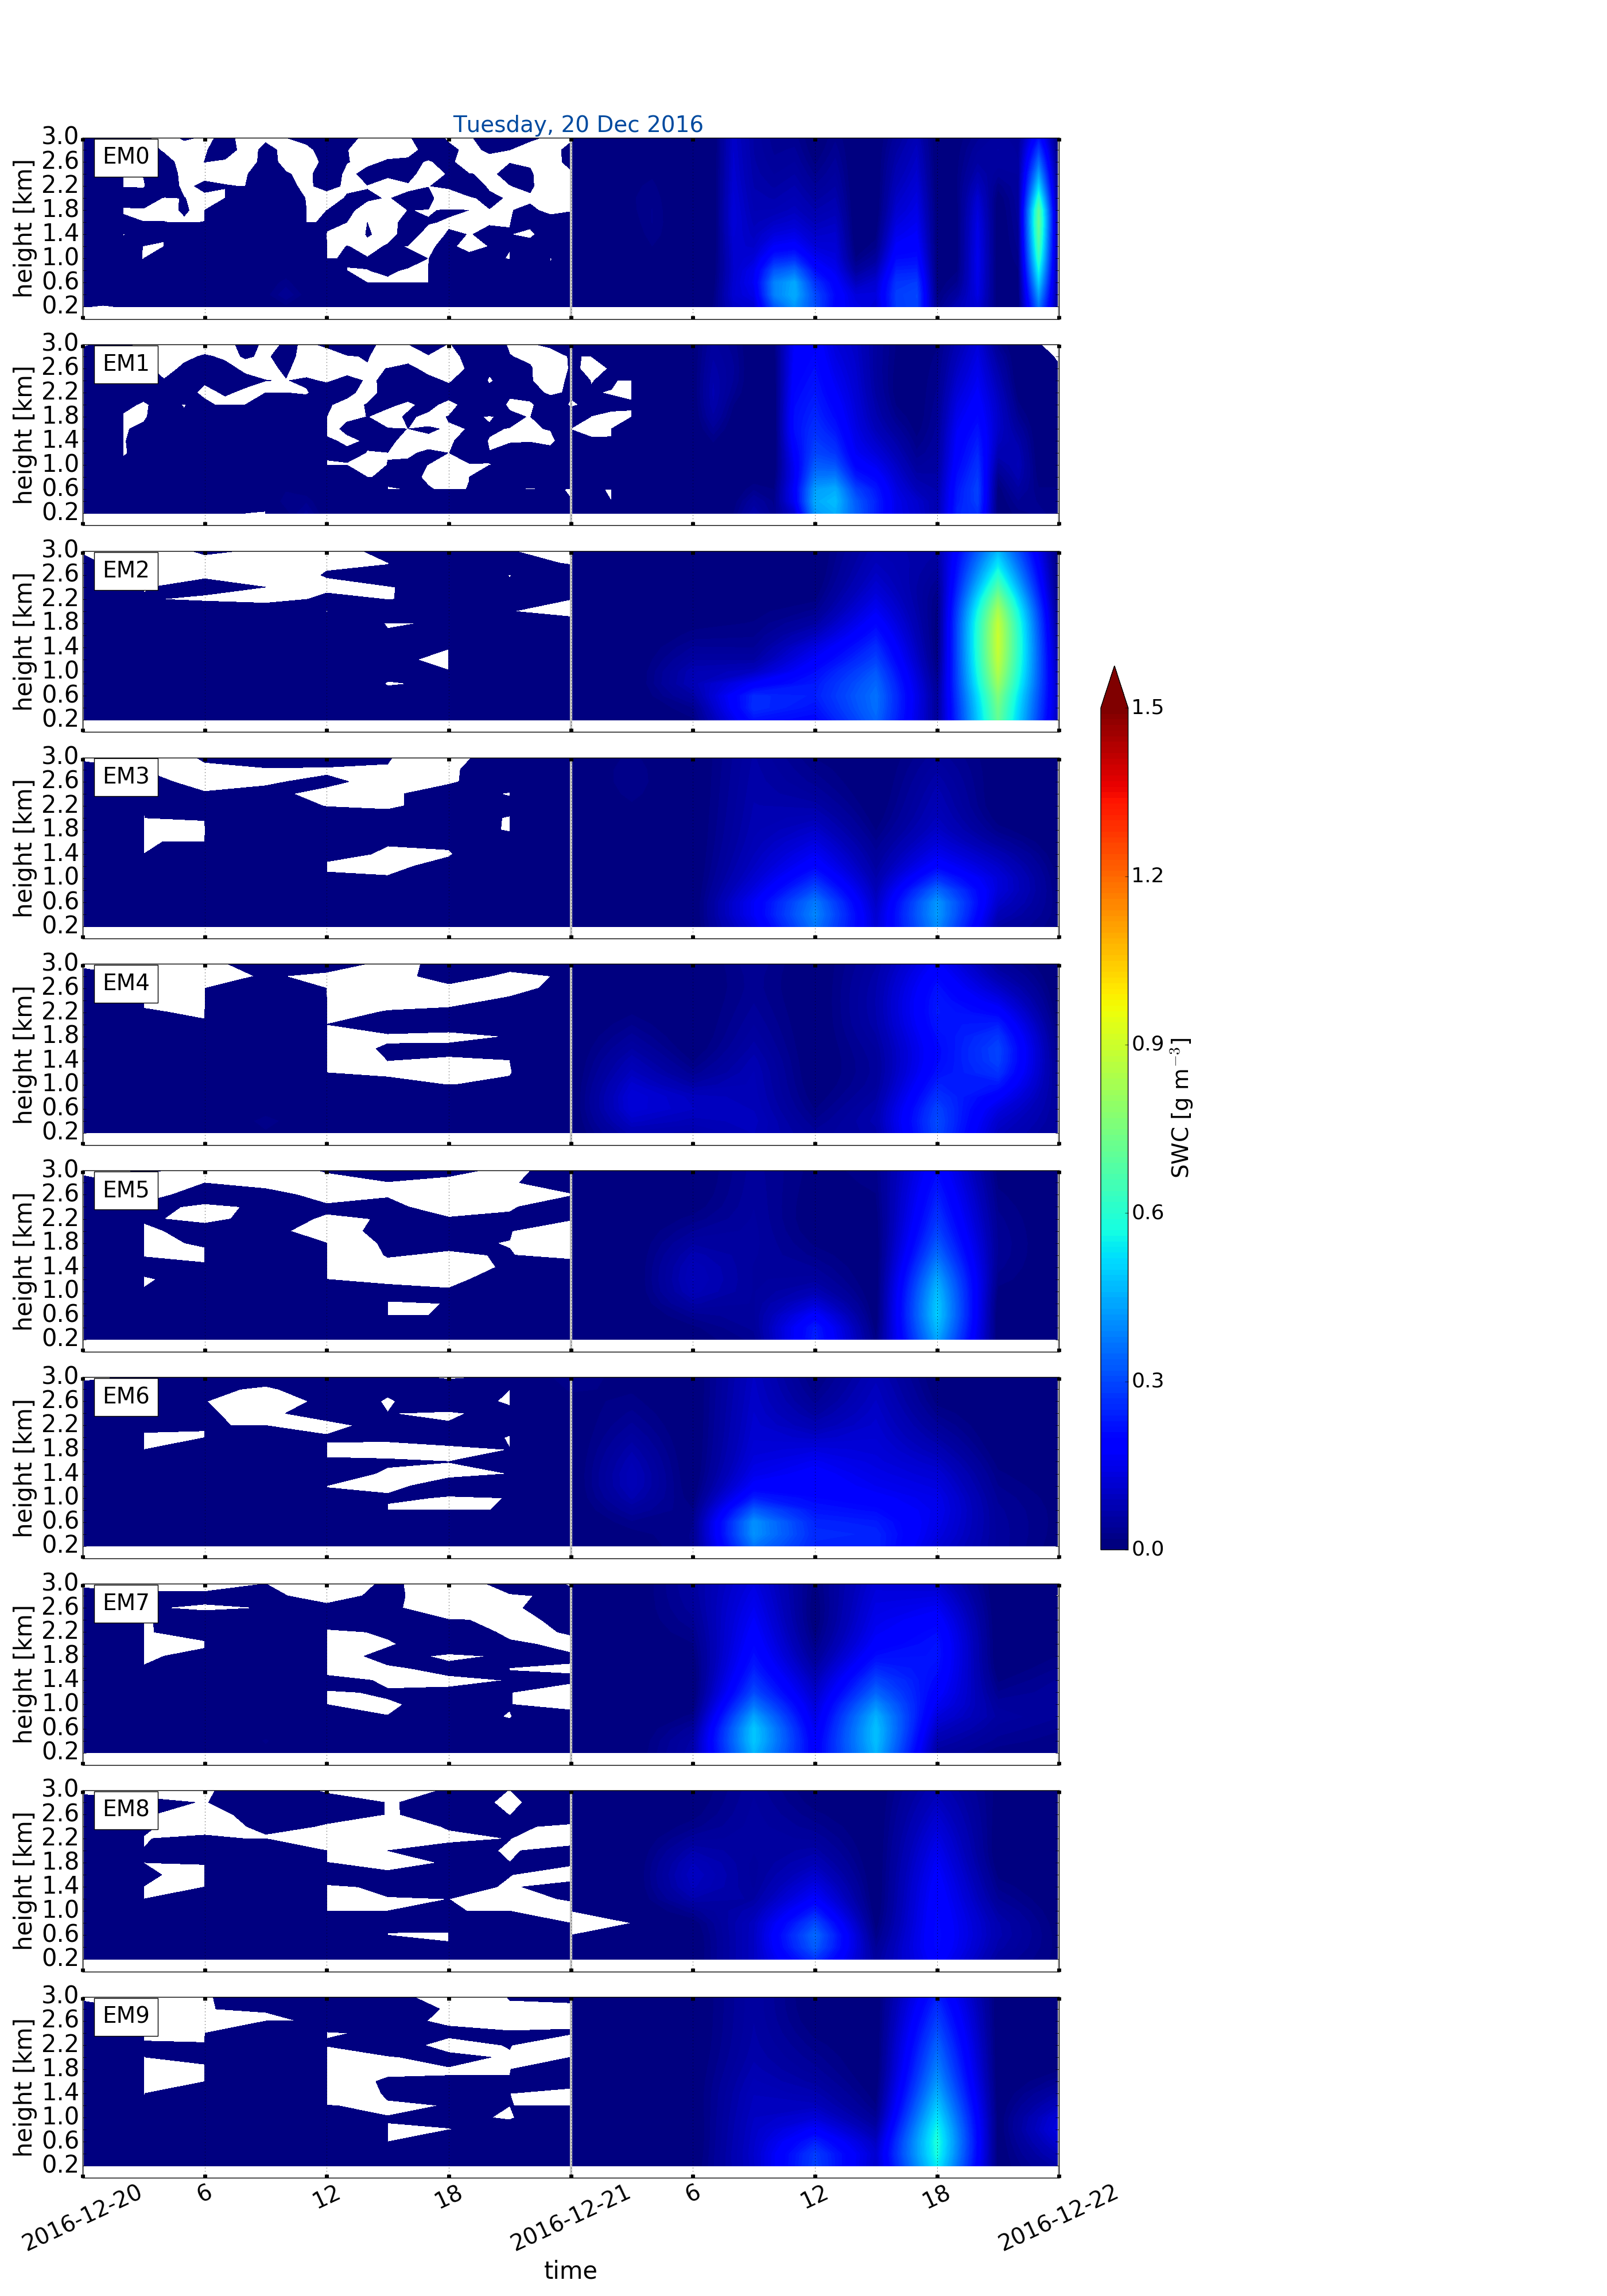
\includegraphics[trim={0cm 0cm 18.3cm 5.1cm},clip,width=0.8\textwidth]{./fig_09EM/20161220}
% 		\caption{initialised Tuesday, \SI{20}{\dec} at 0\SI{0}{\UTC} forecast for \SI{48}{\hour}.}\label{fig:EM09_20}
% 	\end{subfigure}

%      % 21/12
%  		\begin{subfigure}[t]{\textwidth}	
% 		\centering
% 		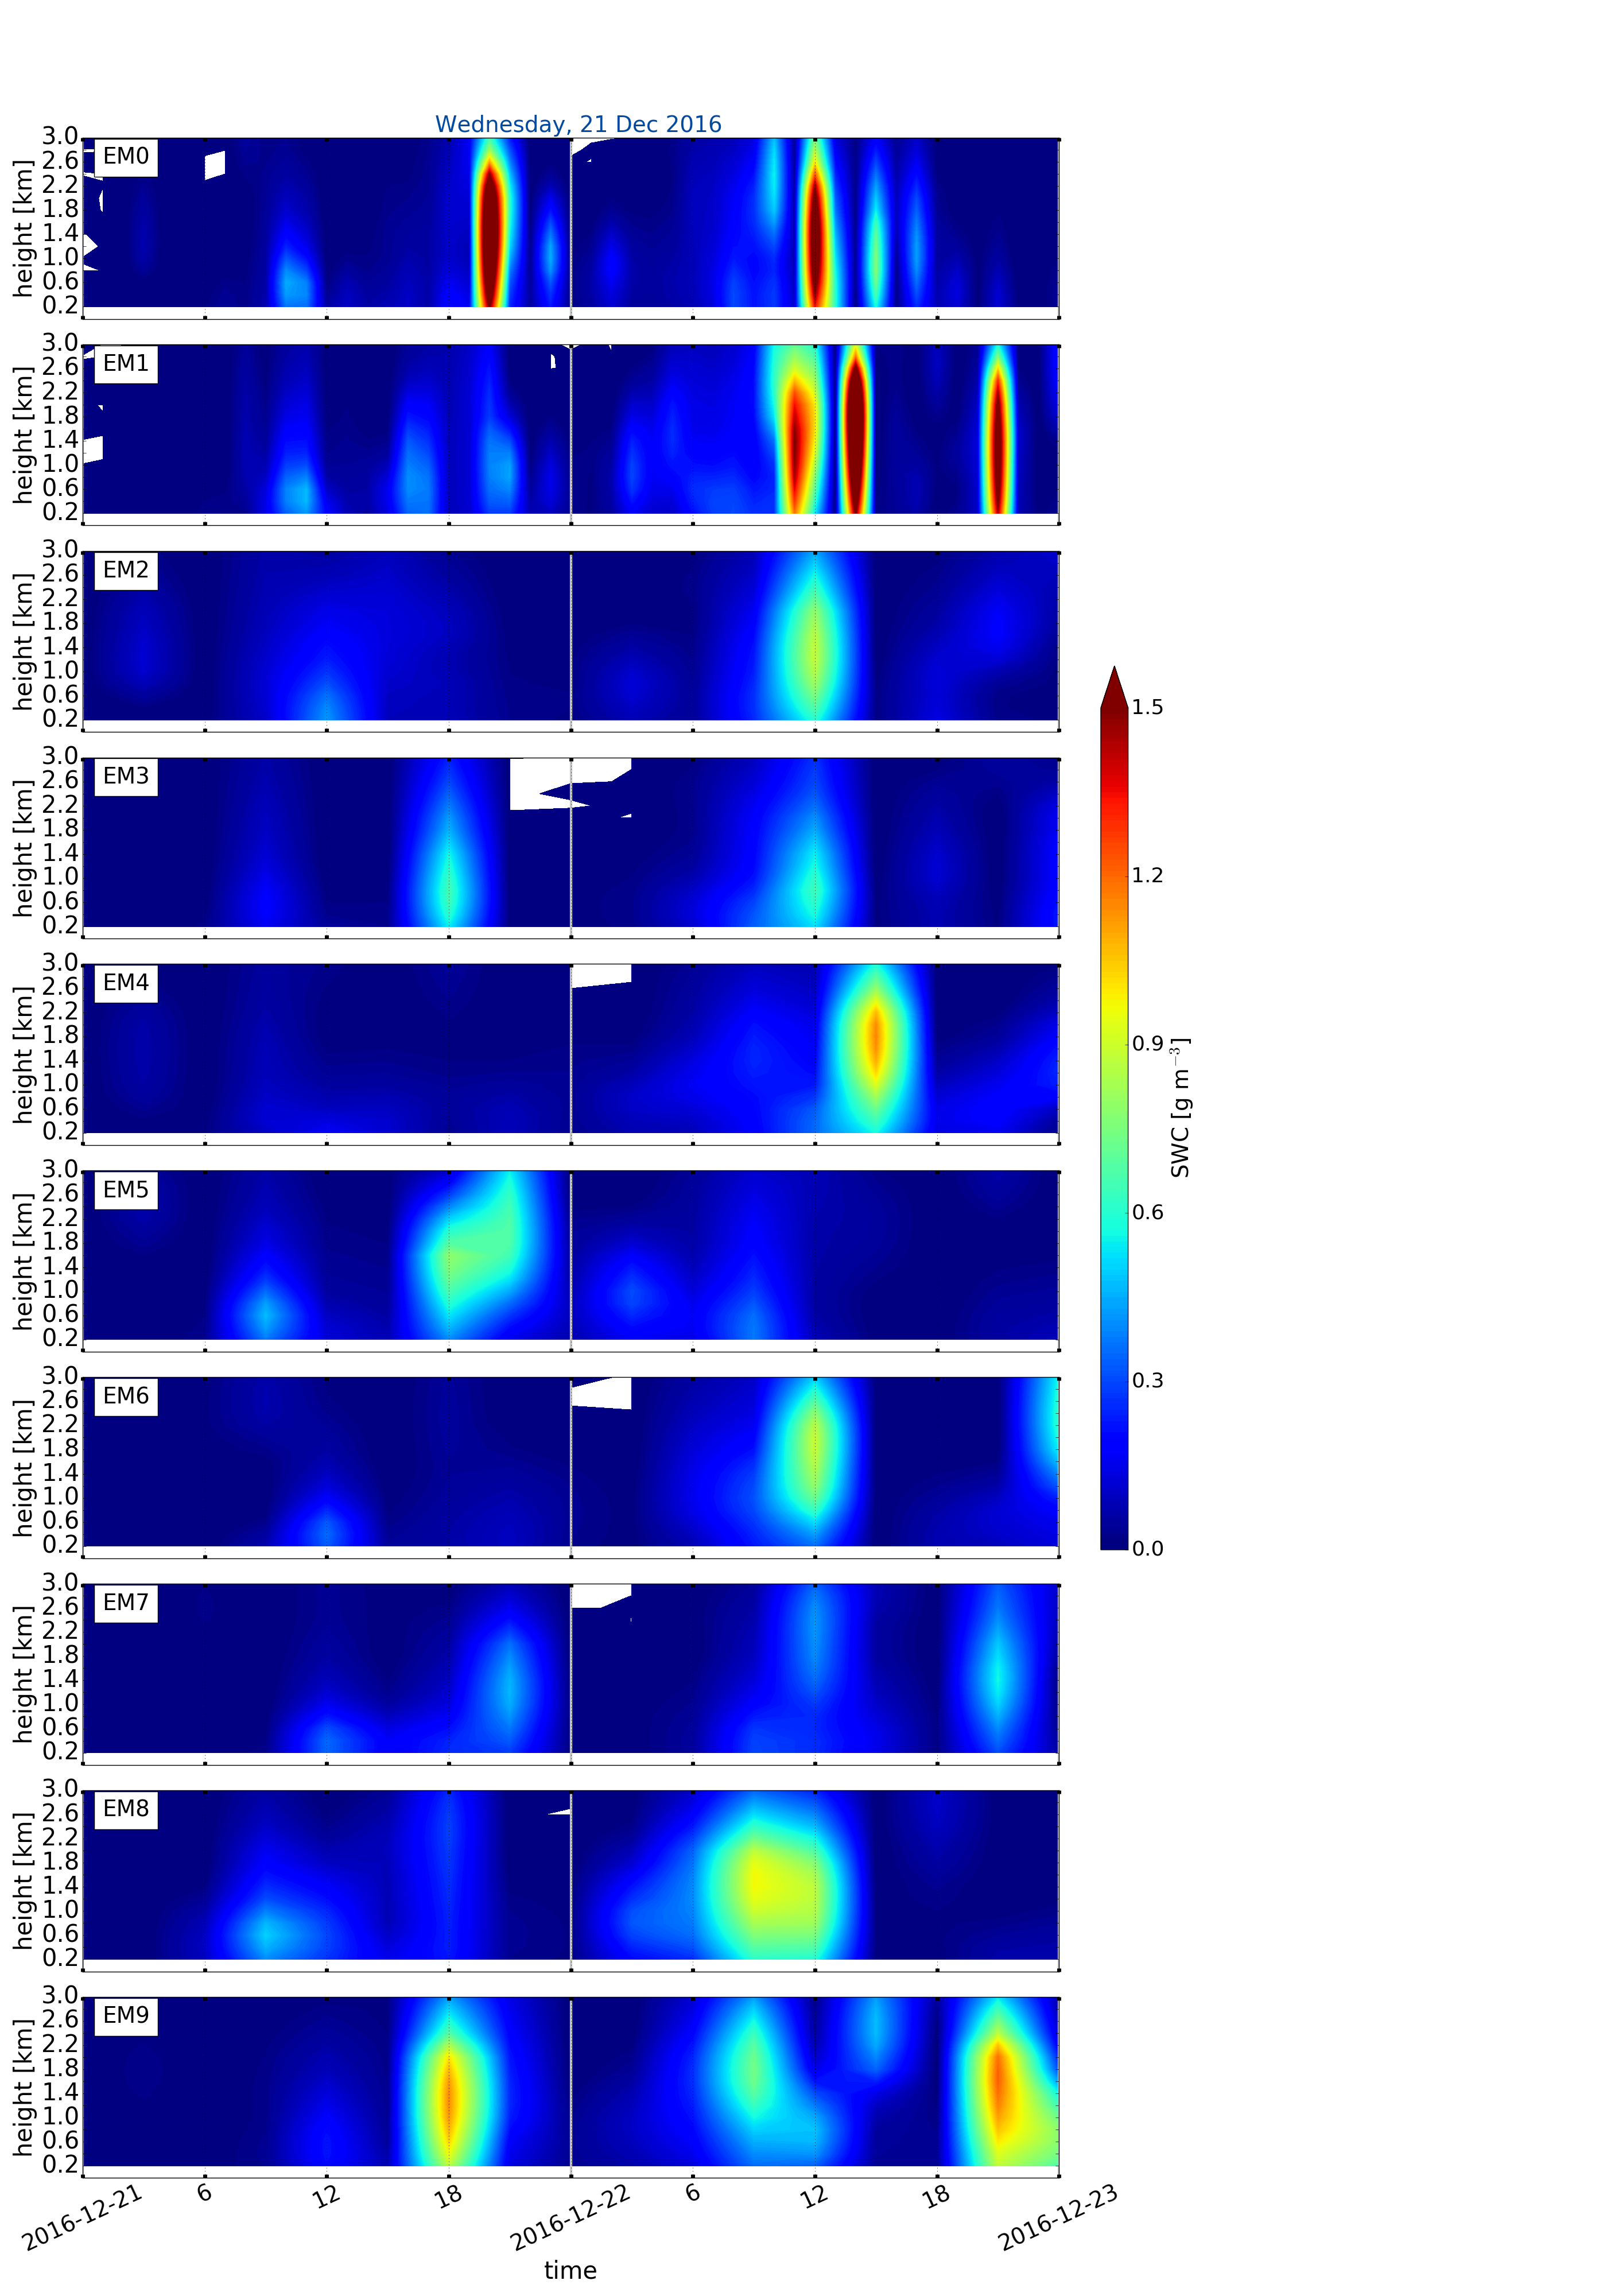
\includegraphics[trim={0cm 0cm 18.3cm 5.1cm},clip,width=0.8\textwidth]{./fig_09EM/20161221}
% 			\caption{SWC of all ensemble members initialised Wednesday, \SI{21}{\dec} at 0\SI{0}{\UTC} forecast for \SI{48}{\hour}.}\label{fig:EM09_21}
% 		\end{subfigure}
% \end{figure}
% \begin{figure}[t]\ContinuedFloat
% 	\centering
% 	% 22/12
% 	\begin{subfigure}[t]{\textwidth}
% 		\centering
% 		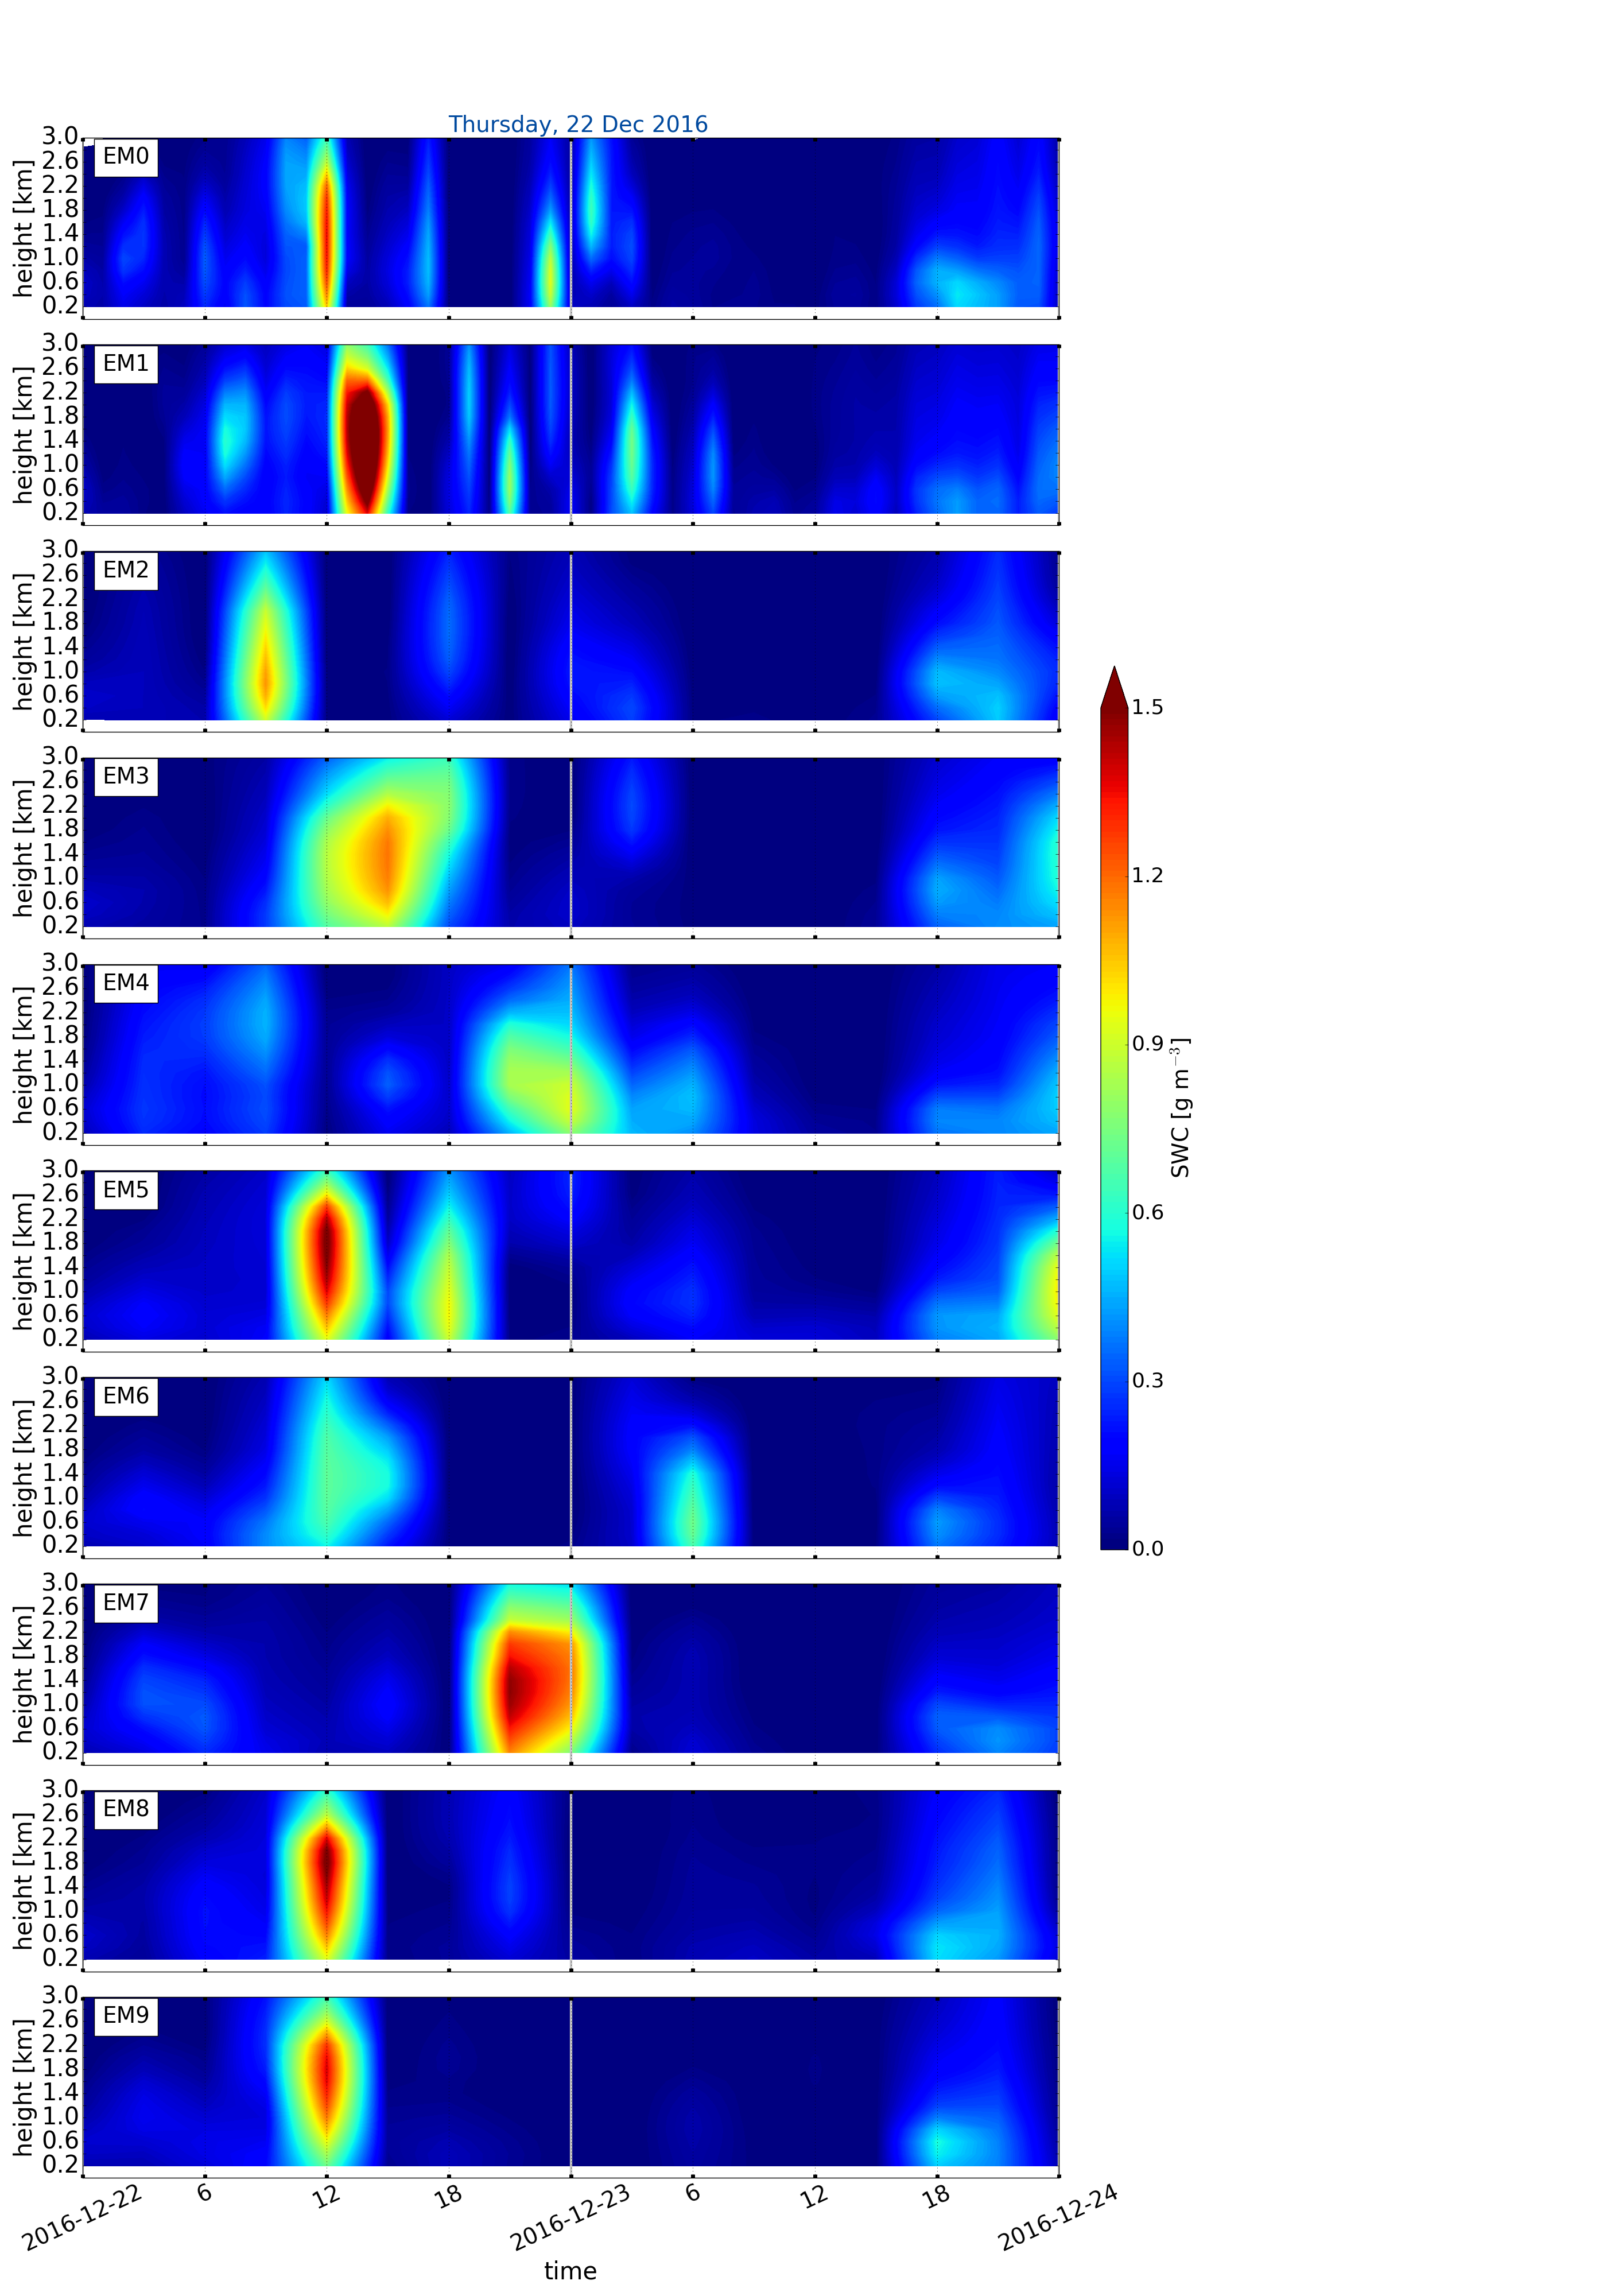
\includegraphics[trim={0cm 0cm 18.3cm 5.1cm},clip,width=0.8\textwidth]{./fig_09EM/20161222}
% 		\caption{SWC of all ensemble members initialised Thursday, \SI{22}{\dec} at 0\SI{0}{\UTC} forecast for \SI{48}{\hour}.}\label{fig:EM09_22}
% 	\end{subfigure}
% \end{figure}
\begin{figure}[h]%\ContinuedFloat
	\centering
	% 23/12
	\begin{subfigure}[t]{\textwidth} 
		\centering
		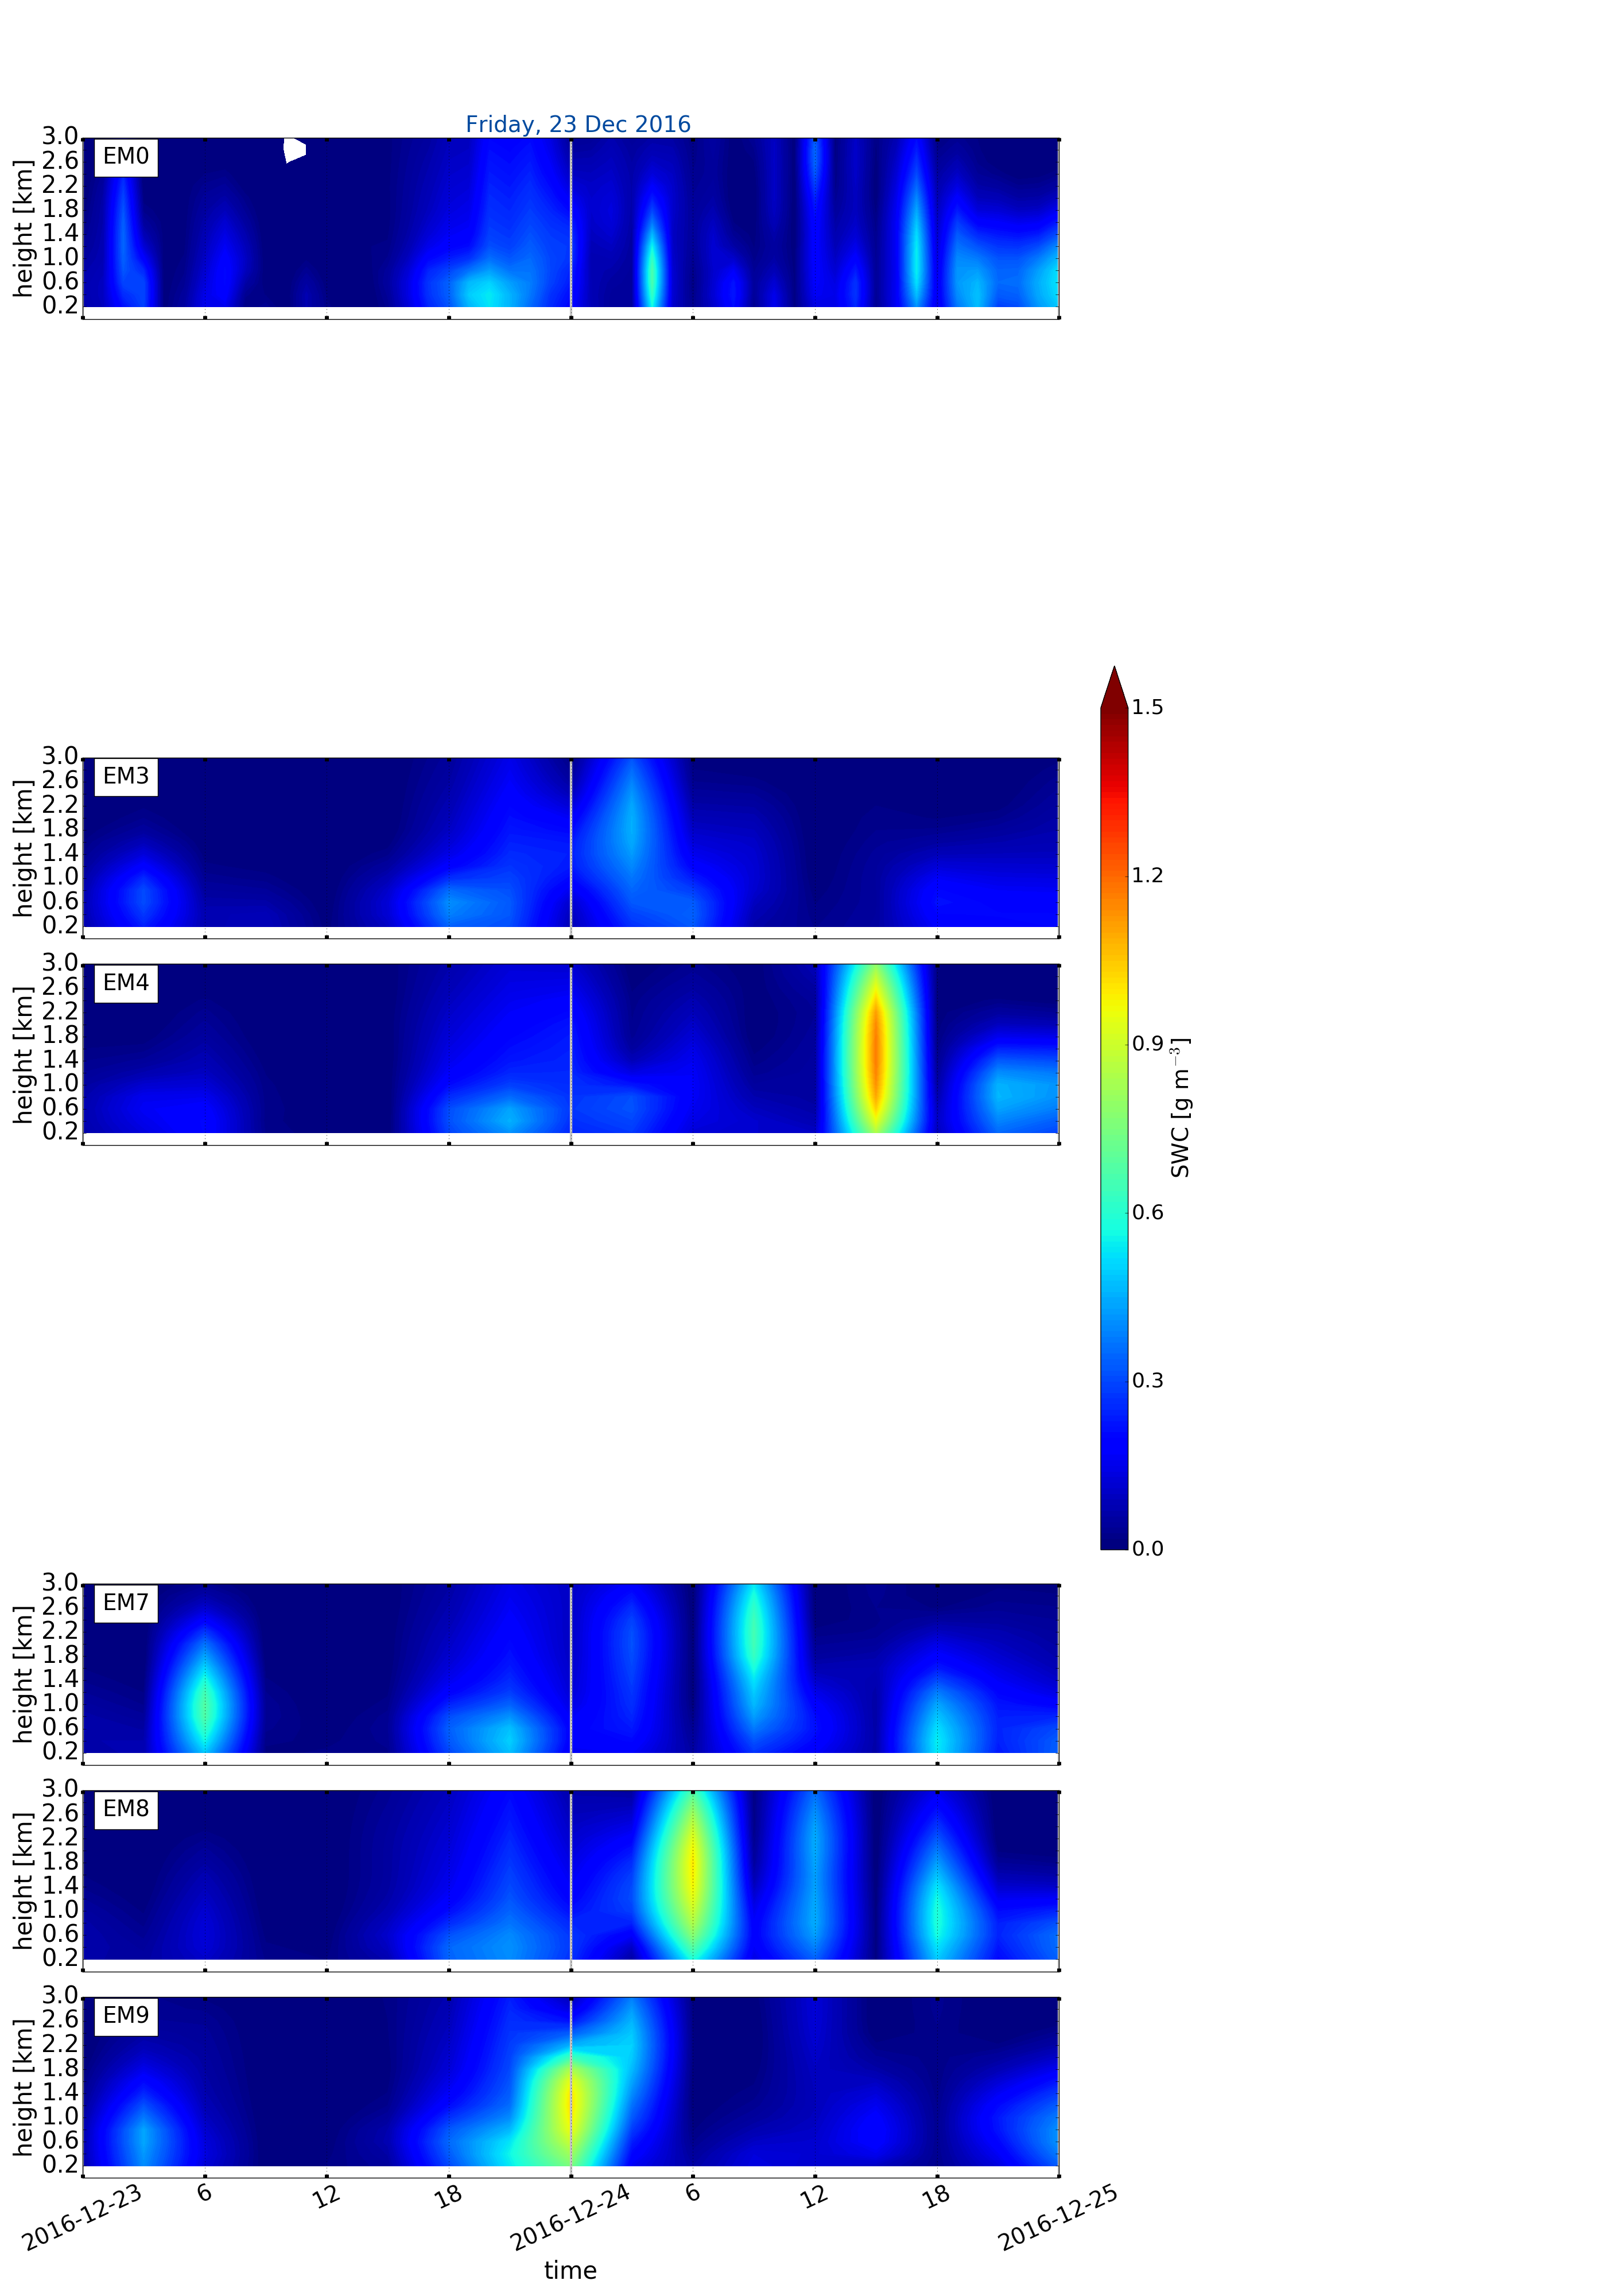
\includegraphics[trim={0cm 0cm 18.3cm 5.1cm},clip,width=0.8\textwidth]{./fig_09EM/20161223}
		\caption{SWC of all ensemble members initialised Friday, \SI{23}{\dec} at 0\SI{0}{\UTC} forecast for \SI{48}{\hour}.}\label{fig:EM09_23}
	\end{subfigure}
	%     % 24/12
	% 		\begin{subfigure}[t]{\textwidth}		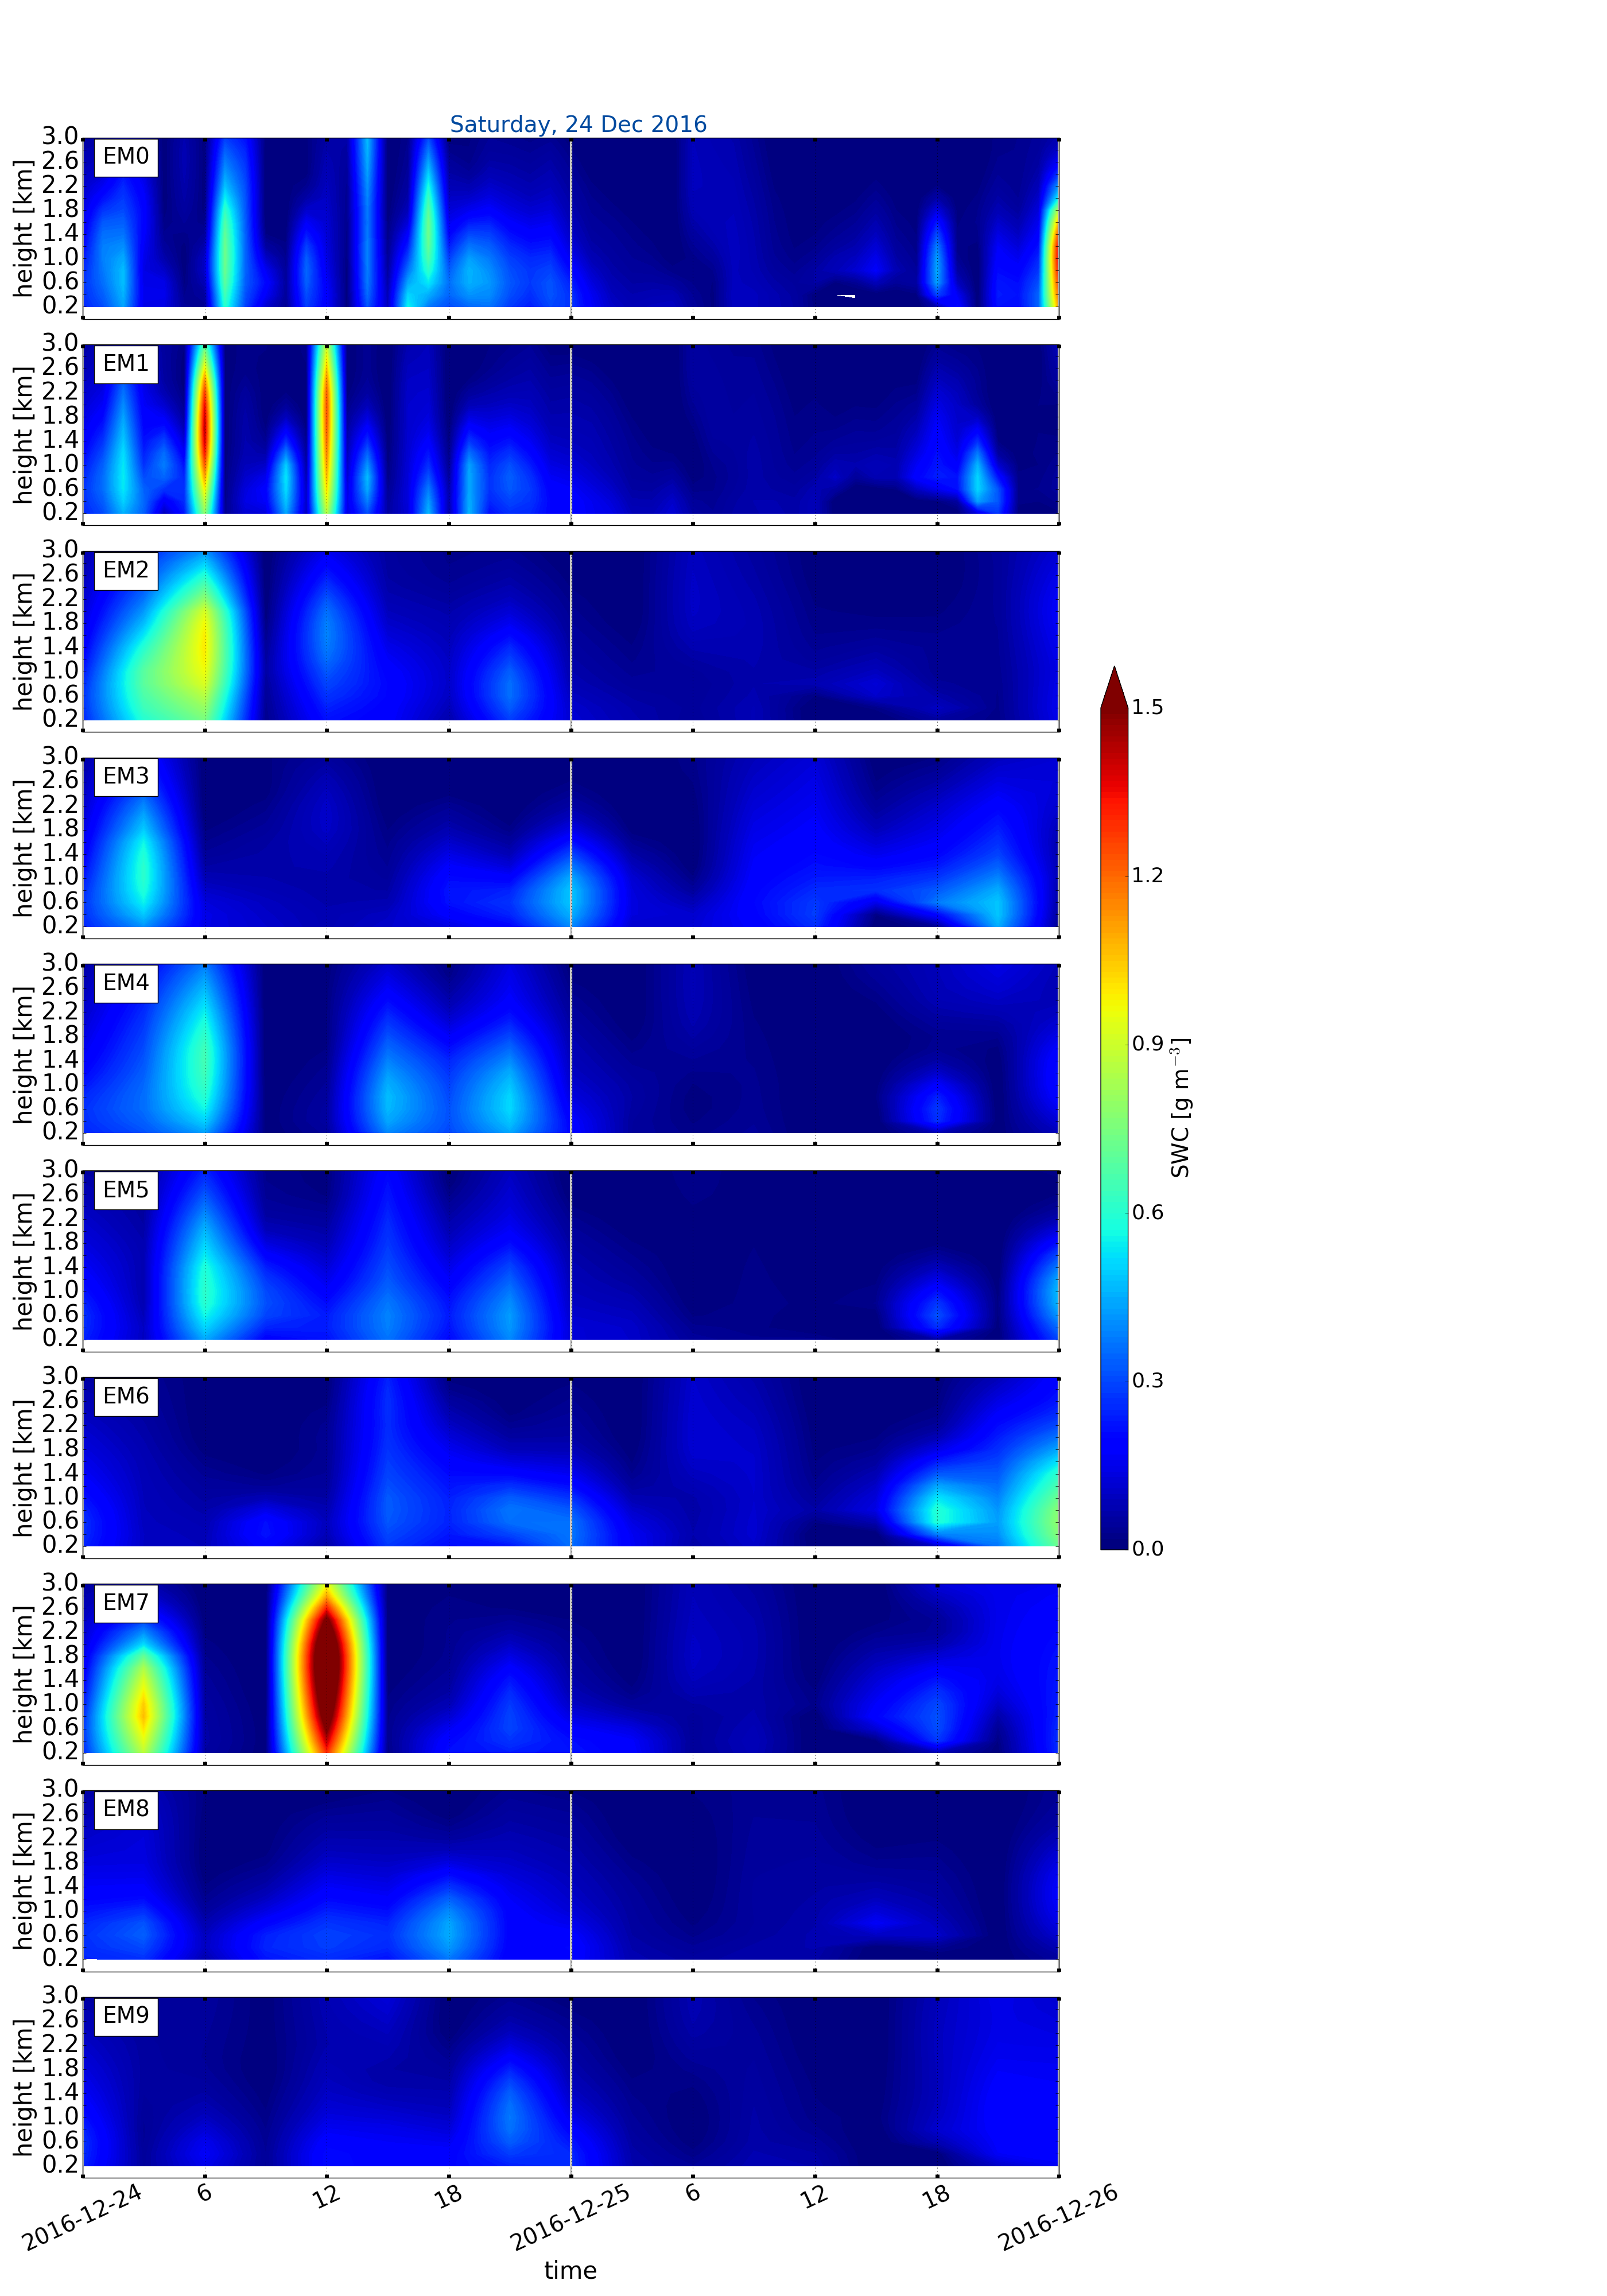
\includegraphics[trim={0cm 0cm 18.3cm 5.1cm},clip,width=0.8\textwidth]{./fig_09EM/20161224}
	% 			\caption{SWC of all ensemble members initialised Saturday, \SI{24}{\dec} at 0\SI{0}{\UTC} forecast for \SI{48}{\hour}.}\label{fig:EM09_24}
	% 		\end{subfigure}
	% 25/12
\end{figure}
\begin{figure}\ContinuedFloat
	\centering
	\begin{subfigure}[t]{\textwidth}
		\centering
		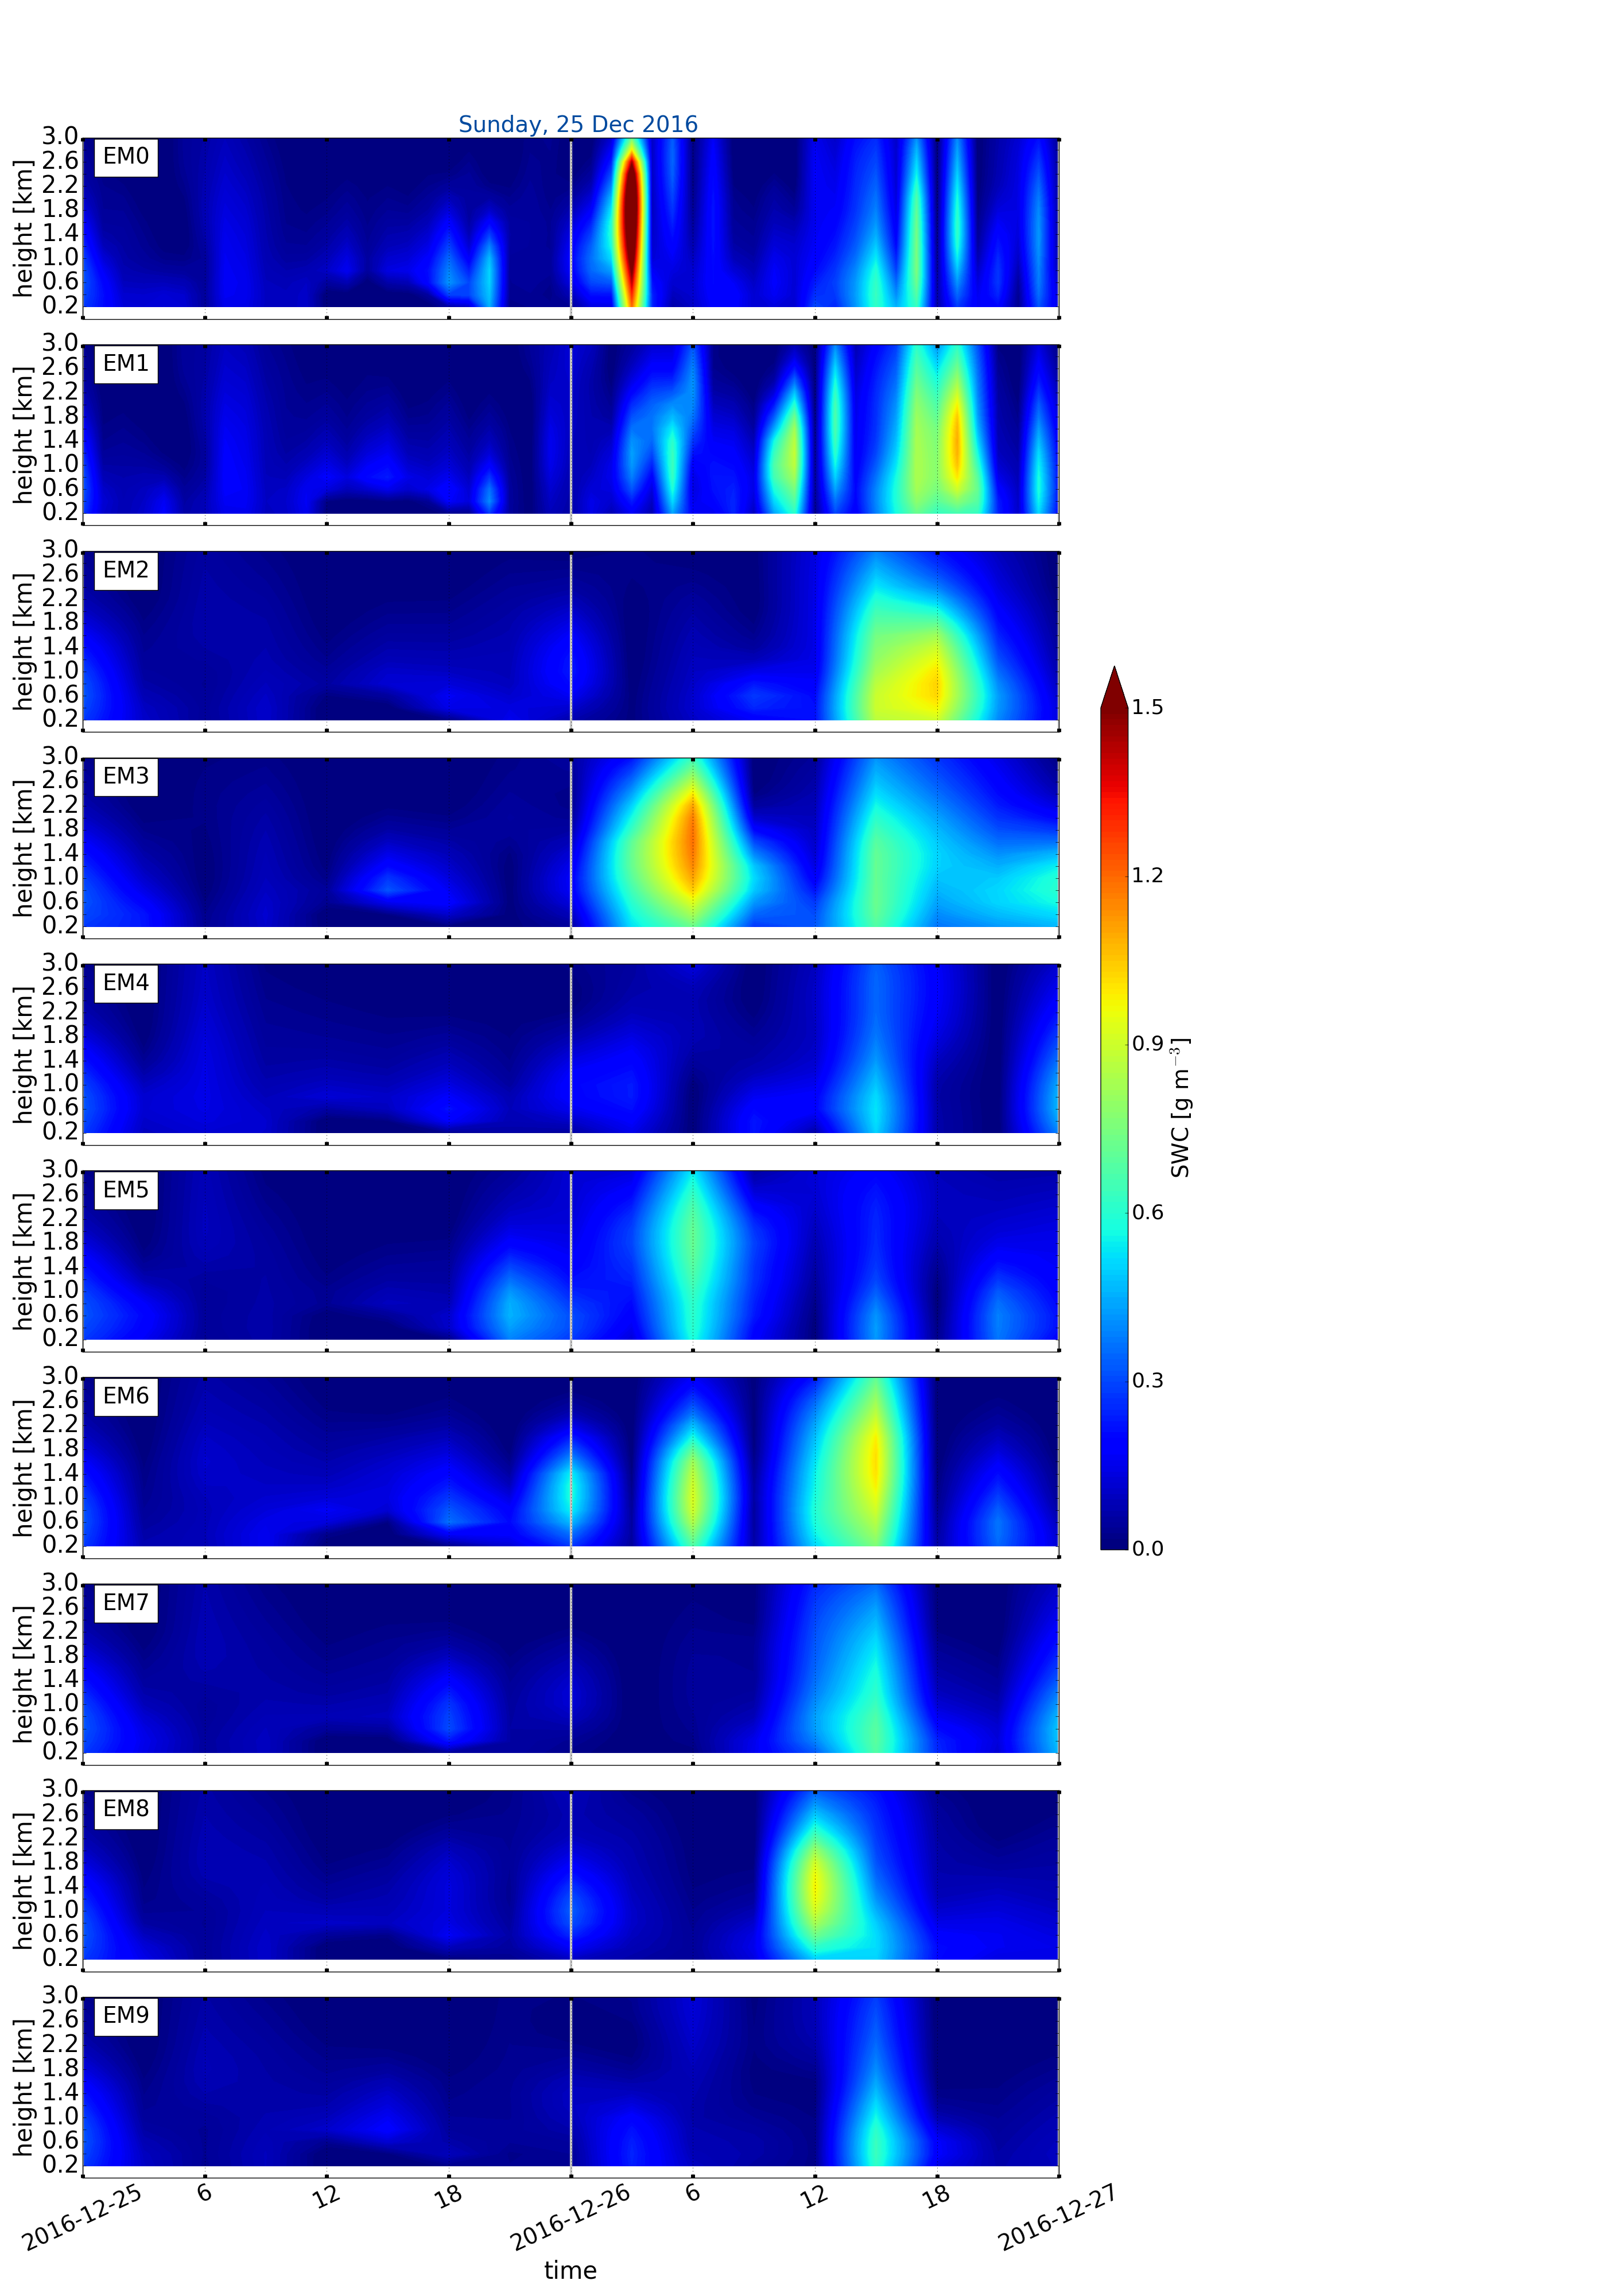
\includegraphics[trim={0cm 0cm 18.3cm 5.1cm},clip,width=0.8\textwidth]{./fig_09EM/20161225}
		\caption{SWC of all ensemble members initialised Sunday, \SI{25}{\dec} at 0\SI{0}{\UTC} forecast for \SI{48}{\hour}.}\label{fig:EM09_25}
	\end{subfigure}
\end{figure}
\begin{figure}[t]\ContinuedFloat
	\centering
	% 26/12
	\begin{subfigure}[t]{\textwidth}	
		\centering
		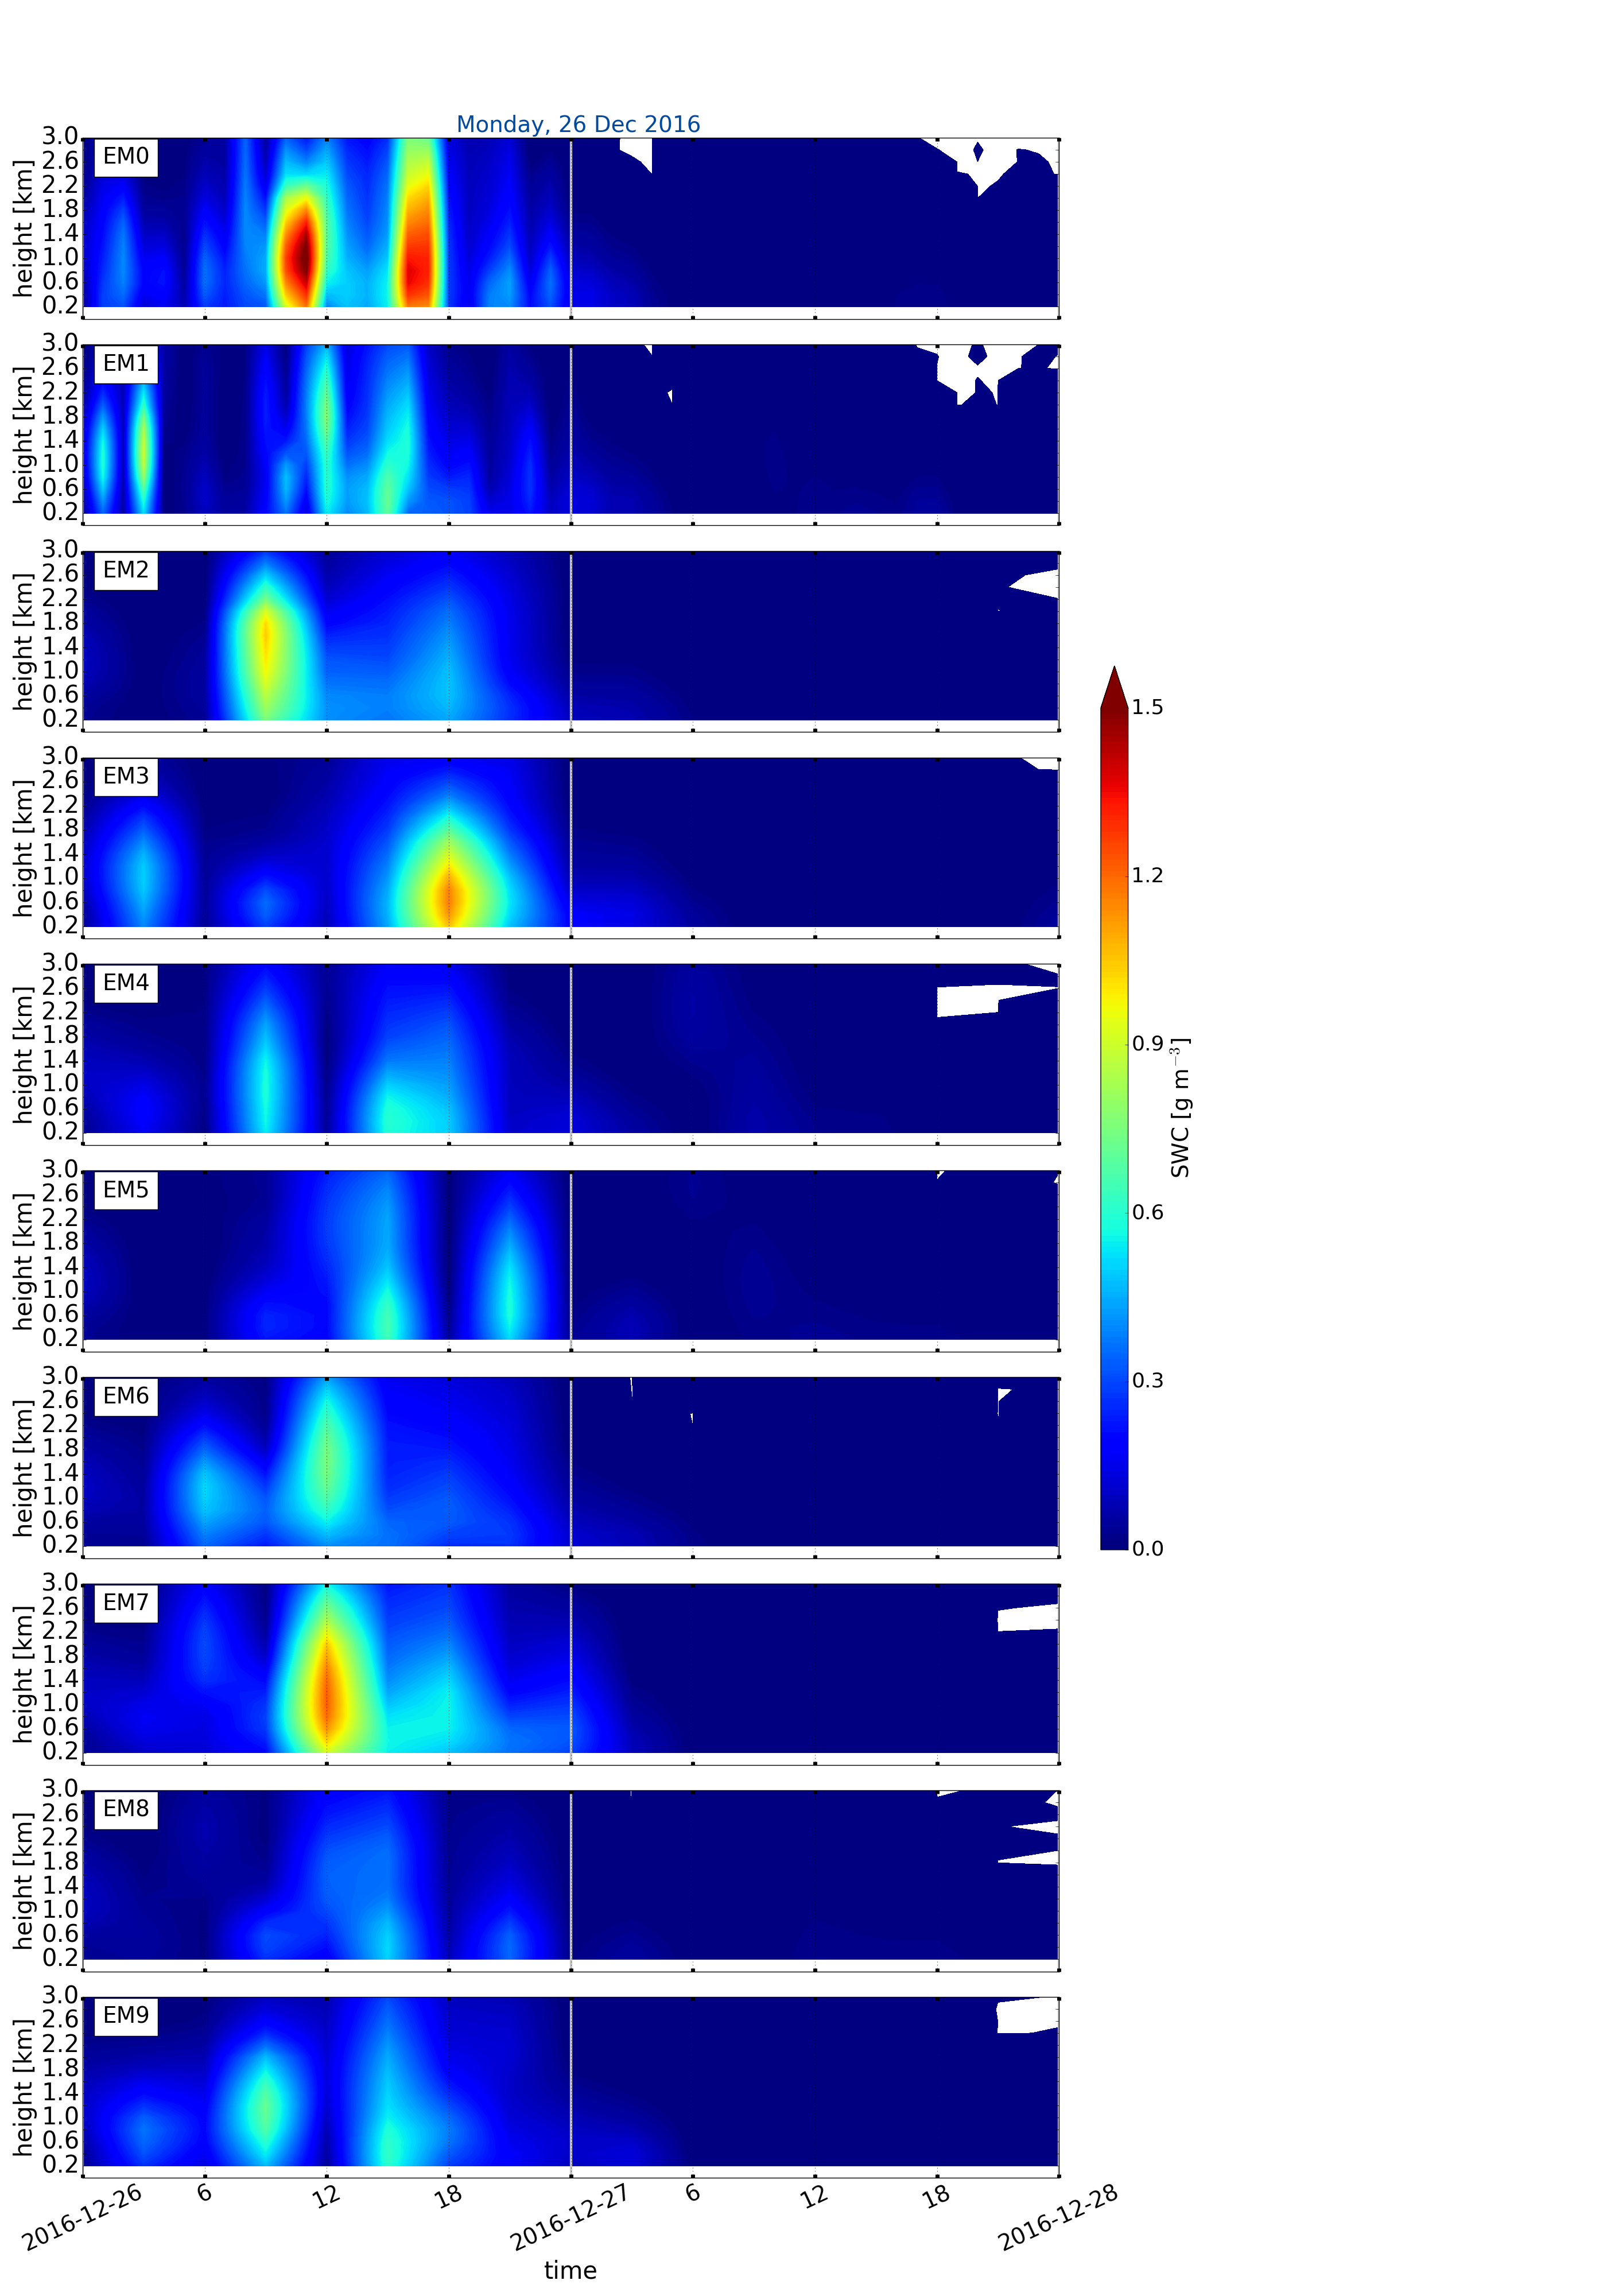
\includegraphics[trim={0cm 0cm 18.3cm 5.1cm},clip,width=0.8\textwidth]{./fig_09EM/20161226}
		\caption{SWC of all ensemble members initialised Monday, \SI{26}{\dec} at 0\SI{0}{\UTC} forecast for \SI{48}{\hour}.}\label{fig:EM09_26}
	\end{subfigure}
	\caption{Vertical SWC of each individual ensemble member from \numrange{0}{9}}\label{fig:EM09}
\end{figure}

%%%%%%%%%%%%%%%%%%%%%%%%%%%%%%%%%%%%%%%%%%%%%%%%%%%%%%%%%%%%%%%%%%%%%%%%%%
